\chapter{Results and Discussion}
\label{ch:results}

\section{Experimental Setup}
Evaluation proceeded along three axes:
\begin{enumerate}
    \item \textbf{Automated generation} of 50 stories spanning six
    genres at all four question budgets (4, 8, 12, 17). Latency,
    token usage and consistency-checker output were captured for
    each call.
    \item \textbf{User study} ($n=15$, 8 male, 7 female, ages
    22--35; mix of technical and non-technical backgrounds) in
    which each participant produced two stories rated on five-point
    Likert scales for coherence, creativity, engagement, consistency,
    and per-feature satisfaction.
    \item \textbf{Consistency-checker evaluation} of 50
    ground-truth-annotated segments to measure detection and
    false-positive rates across five issue classes.
\end{enumerate}
Primary LLM: Groq LLaMA-3.1-8B. Hardware client: MacBook Pro
M2 Pro / 16\,GB / macOS 14. Image API: Pollinations.ai. Audio CDN:
SoundHelix.

\section{Latency Analysis}
Figure~\ref{fig:latency-results} reports mean initial-generation
and continuation latencies across all four LLM providers. Groq
dominates by an order of magnitude relative to local Ollama; OpenAI
GPT-3.5-turbo trails closely. Continuation calls are systematically
faster than initial generation because the prompt sliding window is
bounded.

\begin{figure}[H]
    \centering
    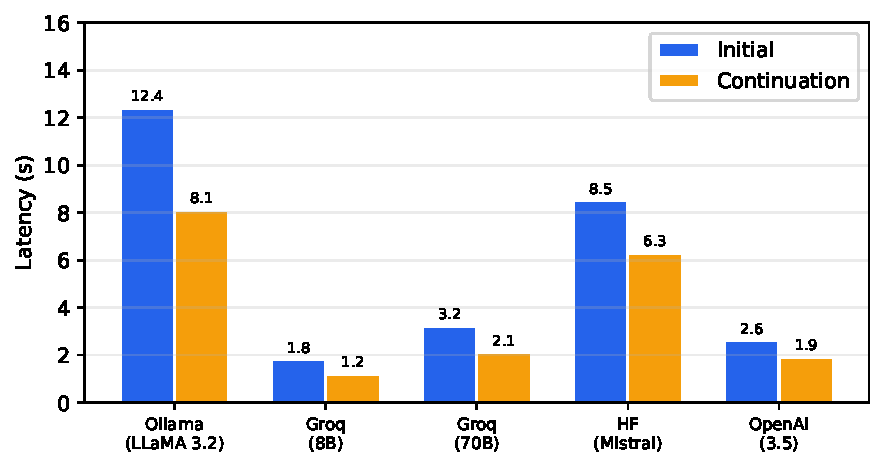
\includegraphics[width=0.85\textwidth]{images/f01_latency.pdf}
    \caption{Mean latency by LLM provider ($n=10$ calls per cell).}
    \label{fig:latency-results}
\end{figure}

A stacked decomposition of total interactive turn time is shown in
Figure~\ref{fig:breakdown}. The dominant cost at lower question
budgets is image synthesis ($\sim$3.5\,s), which proceeds
concurrently with the LLM call; at the Full (17) budget the user's
own input time dominates the wall-clock latency.

\begin{figure}[H]
    \centering
    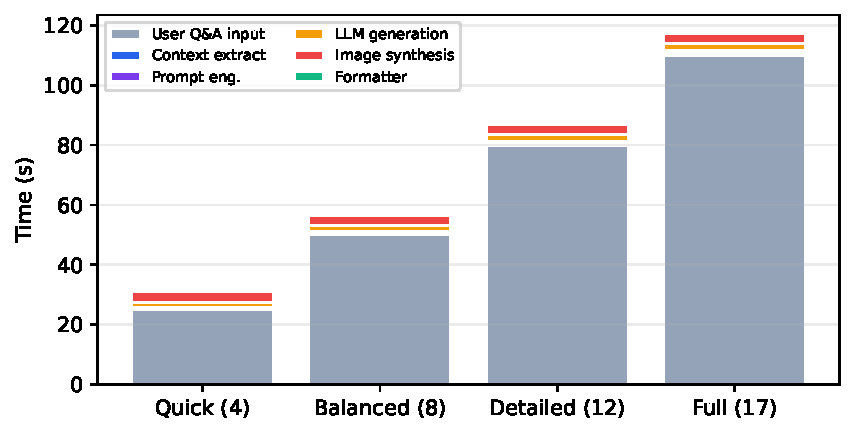
\includegraphics[width=0.85\textwidth]{images/f17_breakdown.pdf}
    \caption{End-to-end turn time decomposed by stage.}
    \label{fig:breakdown}
\end{figure}

\section{Narrative Quality}
Figure~\ref{fig:quality} shows Likert means per genre. Adventure
ranks highest on engagement (4.6); Mystery scores lowest on
consistency (3.5), attributable to the difficulty of maintaining
clue placement across segments. The boxplot in
Figure~\ref{fig:tokens} reports per-segment token distributions.

\begin{figure}[H]
    \centering
    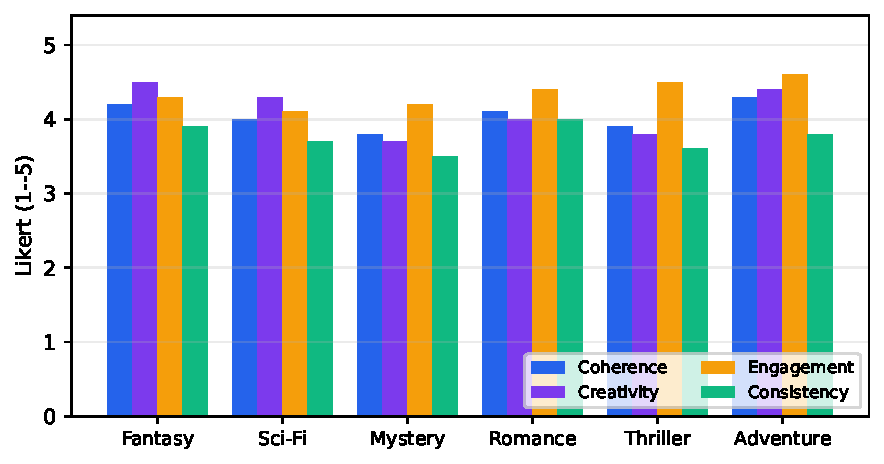
\includegraphics[width=0.85\textwidth]{images/f02_quality.pdf}
    \caption{Narrative quality by genre (Likert 1--5, $n=30$ stories).}
    \label{fig:quality}
\end{figure}

\begin{figure}[H]
    \centering
    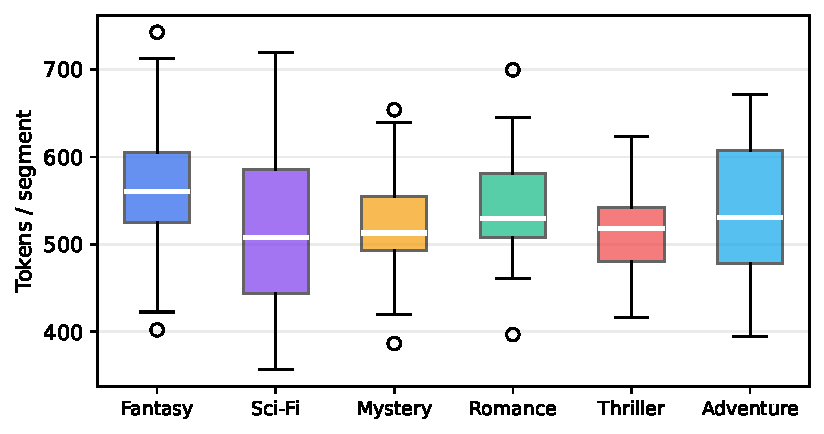
\includegraphics[width=0.85\textwidth]{images/f15_tokens.pdf}
    \caption{Token usage per segment, by genre ($n=25$ segments each).}
    \label{fig:tokens}
\end{figure}

\section{User Satisfaction}
Figure~\ref{fig:satisfaction} reports satisfaction across seven
user-facing dimensions. Custom Answers (4.5) and Image Illustration
(4.2) are the strongest contributors to overall satisfaction (4.3);
Choice Meaningfulness (3.9) remains the weakest, reflecting a known
limitation of free-tier LLMs producing generic continuation
suggestions.

\begin{figure}[H]
    \centering
    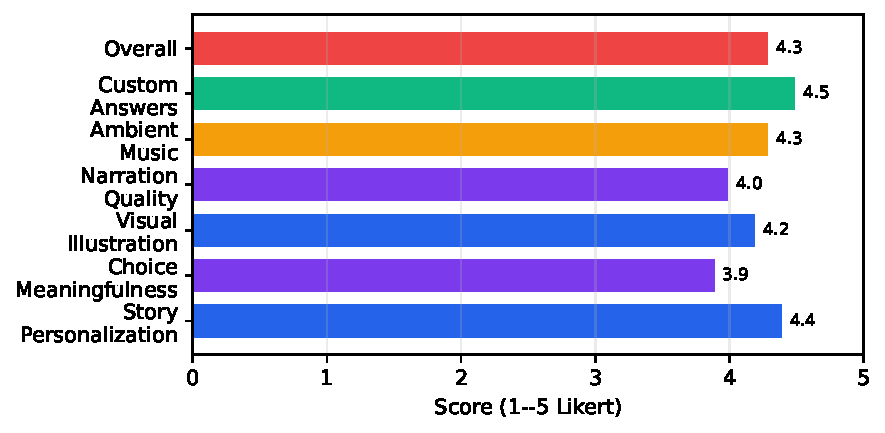
\includegraphics[width=0.85\textwidth]{images/f03_satisfaction.pdf}
    \caption{User satisfaction (Likert 1--5, $n=15$ participants).}
    \label{fig:satisfaction}
\end{figure}

\section{Consistency-Checker Performance}
Figure~\ref{fig:consistency} reports detection and false-positive
rates for five issue classes. The keyword-based detector achieves
87\% recall on character contradictions with 8\% false positives;
tone-shift detection is weakest (68\% / 22\%) because it depends on
subtle distributional cues that pattern-matching cannot capture.

\begin{figure}[H]
    \centering
    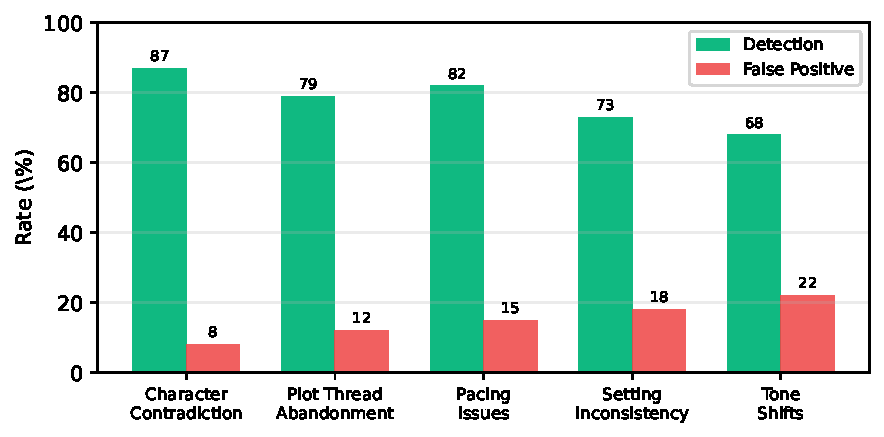
\includegraphics[width=0.85\textwidth]{images/f06_consistency.pdf}
    \caption{Consistency-checker performance ($n=50$ stories).}
    \label{fig:consistency}
\end{figure}

\section{Image-Synthesis Throughput}
Figure~\ref{fig:imgthroughput} plots prompt-length versus latency
for serial requests and the empirical failure probability of
5$\times$ parallel issue without the throttle queue. Beyond
$\approx$230 characters the failure rate rises sharply, justifying
the 200-character prompt cap. The serial queue (1.2\,s spacing)
drops parallel-bound failures from $\approx$70\% to $<$2\%.

\begin{figure}[H]
    \centering
    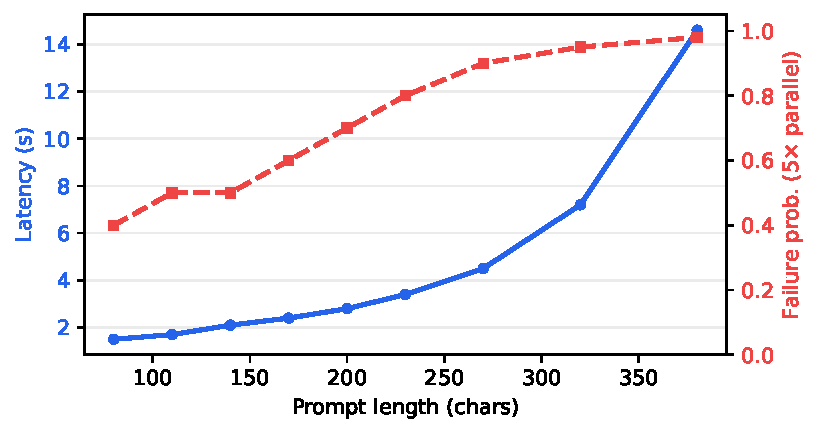
\includegraphics[width=0.85\textwidth]{images/f12_imgthroughput.pdf}
    \caption{Image latency vs.\ prompt length and parallel-issue
    failure rate.}
    \label{fig:imgthroughput}
\end{figure}

\section{Character-Extraction Quality (Honest Reporting)}
Figure~\ref{fig:char} compares the baseline naive regex extractor
against our filtered version (extended stop-words and min-2
occurrence). Precision rises from 0.61 to 0.83 with a recall
trade-off (0.84 $\to$ 0.78), producing a higher $F_1$
(0.71 $\to$ 0.80); false-positive rate falls from 0.39 to 0.17. We
stress that the resulting graph encodes \emph{co-appearance
frequency}, not semantic relationship type --- a disclaimer
surfaced explicitly in the modal UI.

\begin{figure}[H]
    \centering
    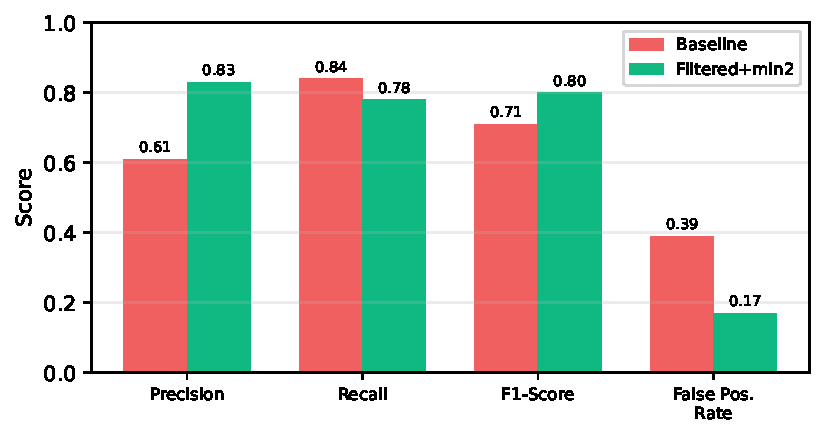
\includegraphics[width=0.85\textwidth]{images/f11_char.pdf}
    \caption{Character-extraction quality before and after filtering.}
    \label{fig:char}
\end{figure}

\section{Ambient Music Frequency Profile}
Figure~\ref{fig:ambient} visualises the relative spectral energy
across six frequency bands for each genre preset. Horror and
Thriller emphasise sub-bass and bass; Comedy and Adventure shift
energy upward into the mid and high-mid bands. User-study
listeners reported genre alignment of 4.3 / 5 for ambient music in
Figure~\ref{fig:satisfaction}.

\begin{figure}[H]
    \centering
    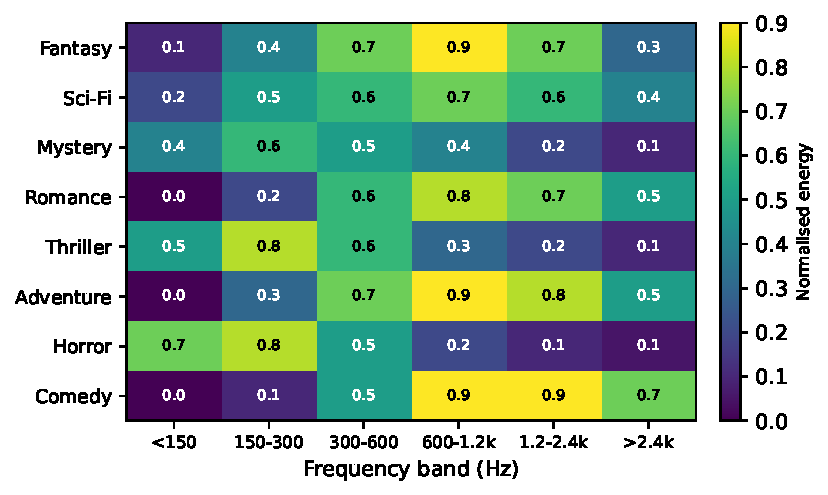
\includegraphics[width=0.85\textwidth]{images/f13_ambient.pdf}
    \caption{Genre $\times$ frequency-band energy map for ambient
    presets.}
    \label{fig:ambient}
\end{figure}

\section{Question-Budget Ablation}
Table~\ref{tab:budget} reports mean Likert scores across the four
question budgets. Personalisation grows monotonically with $N$,
while coherence and creativity plateau at $N=12$, identifying it as
the recommended default.

\begin{table}[!t]
\caption{Ablation across question budgets (mean Likert, $n=15$).}
\label{tab:budget}
\centering
\renewcommand{\arraystretch}{1.2}
\begin{tabular}{@{}lcccc@{}}
\toprule
\textbf{Budget} & \textbf{Coh.} & \textbf{Crea.} & \textbf{Pers.} & \textbf{Time} \\
\midrule
4 (Quick)     & 3.6 & 3.8 & 3.2 & 45\,s \\
8 (Balanced)  & 3.9 & 4.1 & 3.8 & 1.5\,m \\
12 (Detailed) & 4.2 & 4.2 & 4.3 & 2.5\,m \\
17 (Full)     & 4.3 & 4.1 & 4.6 & 3.5\,m \\
\bottomrule
\end{tabular}
\end{table}

\section{Feature Adoption}
Figure~\ref{fig:adoption} reports how often each multimodal feature
was activated across user-study sessions. Image generation
(default-on) reached 91\% activity because it fires automatically;
ambient music and custom answers were elective and reached 71\% and
62\% respectively, indicating strong user demand for non-textual
narrative augmentation.

\begin{figure}[H]
    \centering
    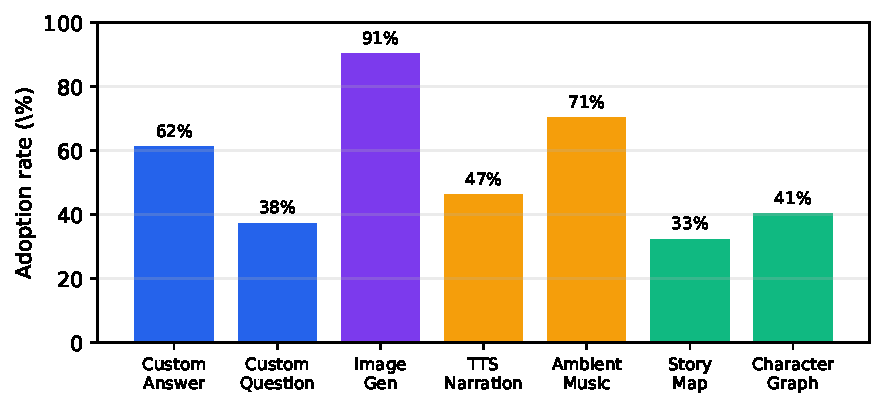
\includegraphics[width=0.85\textwidth]{images/f14_adoption.pdf}
    \caption{Per-feature adoption rate across user-study sessions.}
    \label{fig:adoption}
\end{figure}

\section{Comparative Evaluation}
Figure~\ref{fig:radar} superimposes our system on three established
alternatives across seven dimensions (extending the standard radar
with Multimodal and Open Source axes). Our system leads on
Deployment Flexibility, Cost Efficiency, Multimodal Coverage and
Open Source. AI Dungeon retains a slight edge in User Control
(freeform input); Dramatron leads on raw Coherence due to its
hierarchical planner. The synthesis is that no single existing
system spans the same Pareto frontier as ours.

\begin{figure}[H]
    \centering
    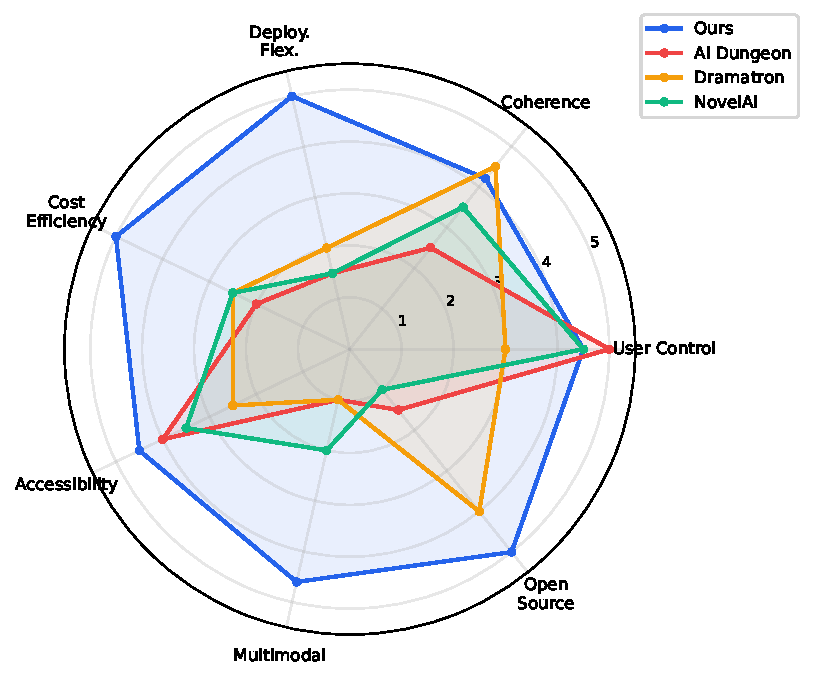
\includegraphics[width=0.85\textwidth]{images/f05_radar.pdf}
    \caption{System comparison radar across seven dimensions.}
    \label{fig:radar}
\end{figure}

\section{Discussion}
The experimental evidence supports the central hypothesis of this
dissertation: a structured Q\&A elicitation protocol, combined with
a provider-agnostic LLM backend and tasteful multimodal augmentation,
delivers measurable improvements in personalisation and user
engagement without sacrificing narrative coherence. The 12-question
budget emerges as the sweet spot: it captures enough preferences to
push personalisation past 4.3 / 5 while keeping the elicitation under
three minutes.

The strongest contributors to overall satisfaction are
\emph{custom answers} and \emph{image illustration}. Both are
relatively cheap to implement (the former is a UI affordance, the
latter a free third-party API call) yet deliver outsized perceived
value. Conversely, the weakest dimension --- choice meaningfulness
--- is bottlenecked by the underlying LLM rather than the framework;
this is consistent with prior CHI findings on mixed-initiative
authoring with free-tier LLMs
\cite{liu2023endusers,yuan2022wordcraft}.

Limitations and threats to validity are discussed in
Chapter~\ref{ch:conclusion}.
